\documentclass[tikz,border=3mm]{standalone}
\usepackage{tikz}

\begin{document}
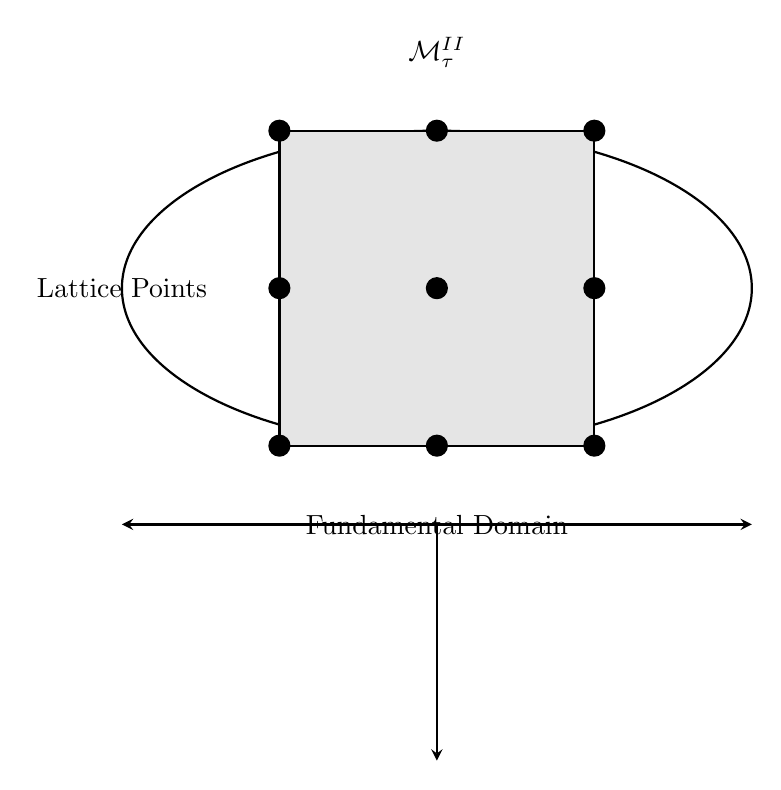
\begin{tikzpicture}[scale=2]
    % Draw the torus
    \draw[thick] (0,0) ellipse (2 and 1);
    \draw[thick] (0,-1) -- (0,1);

    % Draw the fundamental domain
    \draw[thick, fill=gray!20] (-1,-1) rectangle (1,1);

    % Draw the lattice points
    \foreach \x in {-1,...,1}{
        \foreach \y in {-1,...,1}{
            \fill (\x,\y) circle (2pt);
        }
    }

    % Labeling
    \node at (0,1.5) {\(\mathcal{M}^{\text{II}}_{\tau}\)};
    \node at (0,-1.5) {Fundamental Domain};
    \node at (-2,0) {Lattice Points};

    % Arrows indicating direction
    \draw[-stealth, thick] (0,-1.5) -- (-2,-1.5);
    \draw[-stealth, thick] (0,-1.5) -- (2,-1.5);
    \draw[-stealth, thick] (0,-1.5) -- (0,-3);
\end{tikzpicture}
\end{document}